\documentclass[xcolor={dvipsnames}]{beamer}
\mode<presentation>{\usetheme{boxes}}
\usecolortheme{default}
\setbeamertemplate{navigation symbols}{}%remove navigation symbols

\setbeamerfont{frametitle}{size=\Large}

%\setbeamercolor{structure}{fg=beamer@blendedblue}



\setbeamertemplate{bibliography item}{\insertbiblabel}

\setbeamercolor{bibliography entry author}{fg=black}
\setbeamercolor{bibliography entry title}{fg=black} 
\setbeamercolor{bibliography entry location}{fg=black} 
\setbeamercolor{bibliography entry note}{fg=black}  

\usepackage[style=numeric,sorting=ydnt,maxnames=1,defernumbers=true, firstinits=true]{biblatex}
\renewbibmacro{in:}{}
\ExecuteBibliographyOptions{sorting=ydnt}

%\addbibresource{./jlescSummerSchool_checkpointing.bib}

\makeatother
\setbeamertemplate{footline}
{
  \leavevmode%
  \hbox{%
    %% \begin{beamercolorbox}[wd=.2\paperwidth,ht=2.25ex,dp=1ex]{date in head/foot}%
    %%   \usebeamerfont{date in foot}
    %% \end{beamercolorbox}%
  %%   \begin{beamercolorbox}[wd=.6\paperwidth,ht=2.25ex,dp=1ex, center]{date in head/foot}%
  %%     \usebeamerfont{date in foot}\insertshortdate
  %% \end{beamercolorbox}%
  \begin{beamercolorbox}[wd=\paperwidth,ht=2.25ex,dp=1ex]{date in head/foot}%
    \usebeamerfont{date in foot}\hfill
    {\scriptsize\insertframenumber{}}\hspace*{2ex}
  \end{beamercolorbox}}%
  \vskip0pt%
}
\makeatletter



\usepackage[utf8]{inputenc}
%\usepackage[T1]{fontenc}
%\usepackage[francais]{babel}
\usepackage{hyperref}
\usepackage{url}
\usepackage{pifont}
\usepackage{changepage}
\usepackage{listings}
\lstset{basicstyle=\ttfamily,
  showstringspaces=false,
  commentstyle=\color{black},
  keywordstyle=\color{black}
}

\usepackage{fancyvrb}
\usepackage{multirow}
\usepackage{tabu} 
\usepackage{colortbl}

\usepackage{marvosym}

\usepackage{eurosym}

%\usepackage{gitdags}
\usepackage{comment}

\usepackage{pdfpages}
\setbeamercolor{background canvas}{bg=}


\usepackage{perpage} %the perpage package
\MakePerPage{footnote}



\definecolor{beamer@blendedblue}{RGB}{0,102,204}

\definecolor{beamer@lightgray}{RGB}{238,238,224}


\definecolor{itemorange}{RGB}{255,114,0}


\definecolor{myorange}{RGB}{255,103,0}


\setbeamertemplate{itemize items}[circle]
\setbeamertemplate{itemize subitem}[triangle]


\setbeamercolor{itemize item}{fg=beamer@blendedblue}
\setbeamercolor{itemize subitem}{fg=gray}


\newcommand<>{\Blue}[1]{{\color#2{beamer@blendedblue}#1}}
%\newcommand<>{\Orange}[1]{{\color#2{BurntOrange}#1}}
\newcommand<>{\Orange}[1]{{\color#2{myorange}#1}}
\newcommand<>{\Alert}[1]{{\Orange{\textbf{#1}}}}


\newcommand{\largeskip}{\vspace{0.6cm}}
\newcommand{\hugeskip}{\vspace{1cm}}



\usepackage{tikz}
\usetikzlibrary{%
decorations.pathreplacing,%
decorations.pathmorphing,%
decorations.shapes,%
decorations.text,%
decorations.markings,%
shapes,%
shapes.callouts,%
shadows,%
arrows,
calc,%
positioning,%
chains,%
backgrounds,%
fit, %
fadings}

\tikzset{
    invisible/.style={opacity=0},
    visible on/.style={alt={#1{}{invisible}}},
    alt/.code args={<#1>#2#3}{%
      \alt<#1>{\pgfkeysalso{#2}}{\pgfkeysalso{#3}} % \pgfkeysalso doesn't change the path
    },
}


\tikzset{
    colornode/.style={
        outer sep=0pt, fill=#1!67, %text height=2ex, text depth=.5ex
    },
    cpu/.style={
        diamond, fill=gray!30, aspect=3, name=CPU#1,
        node contents={$\text{CPU}_{#1}$},
    },
    thread/.style={fill=#1!67,
        minimum width=5ex, minimum height=1.25em},
    tick/.style={very thin},
}



\newcommand{\email}[1]{\href{mailto:#1}{\nolinkurl{#1}}}

\newcommand{\xmark}{\ding{55}}


\AtBeginPart{
  %\frame{\partpage}
  \frame{
    \frametitle{Agenda}
    \small
    \tableofcontents[part=\insertpartnumber,
    sectionstyle=show,
    subsectionstyle=hide,
    subsubsectionstyle=hide]
  }
}

\AtBeginSection[]
{
  \begin{frame}
    \frametitle{Agenda}
    \small
    \tableofcontents[
    sectionstyle=show/shaded,
    subsectionstyle=show/show/hide,
    subsubsectionstyle=hide]
  \end{frame}
}

\AtBeginSubsection[]{
  \mode<presentation>{
    \frame{\tableofcontents[
      sectionstyle=show/hide,
      subsectionstyle=show/shaded/hide,
      subsubsectionstyle=show/show/hide]
    }
  }
}


\date[\the\year]{\the\year}

\newcommand{\shellcmd}[1]{\indent\indent\texttt{\footnotesize\$ #1}}


\title[]{Cloud Computing}
\subtitle{Le numérique et l'environnement}

%Thomas ROPARS : \url{https://tropars.github.io/teaching/},
%\url{https://roparst.gricad-pages.univ-grenoble-alpes.fr/cloud-tutorials/m2gi-devops/}}}


\author[]{\\Danilo Carastan dos Santos
  \\ \vspace{0.5cm} \email{danilo.carastan-dos-santos@univ-grenoble-alpes.fr}}

\definecolor{mybrown}{RGB}{205,133,63}
\definecolor{myblue}{RGB}{28,134,238}

\let\Red=\alert
\newcommand<>{\green}[1]{{\color#2{green!70!black}#1}}
\newcommand<>{\blue}[1]{{\color#2{blue!100!black!100}#1}}
\definecolor{darkgreen}{rgb}{0,0.5,0}

\newcommand\myvdots{{\smash[b]\strut\smash[t]\vdots}}


\usepackage{boxedminipage}
\newenvironment{boitecode}[1]{
    \begin{boxedminipage}{\linewidth}      
%\begin{beamerboxesrounded}[shadow=true,lower=lightex,upper=medex]{#1}
    #1
    \begin{semiverbatim}
}{   \end{semiverbatim}\vspace{-1.5\baselineskip}
    \end{boxedminipage}
%  \end{beamerboxesrounded}
}


\begin{document}


\begingroup
\setbeamercolor{titlelike}{bg=beamer@lightgray, fg=black}
\begin{frame}
\titlepage
\end{frame}
\endgroup

%\begin{frame}{Contenu}
%    \begin{itemize}
%        \item Motivation (le mythe du dématérialisé)
%        \item Impact environnemental et durabilité
%        \item Catégorie d'impacts (ordre, scope)
%        \item Indicateurs d'impact 
%        \item Cycles de vie
%        \item Effet rebond
%        \item Réflexion sur les eco-gestes        
%    \end{itemize}
%\end{frame}

%\begin{frame}{Le constat}
%    \centering 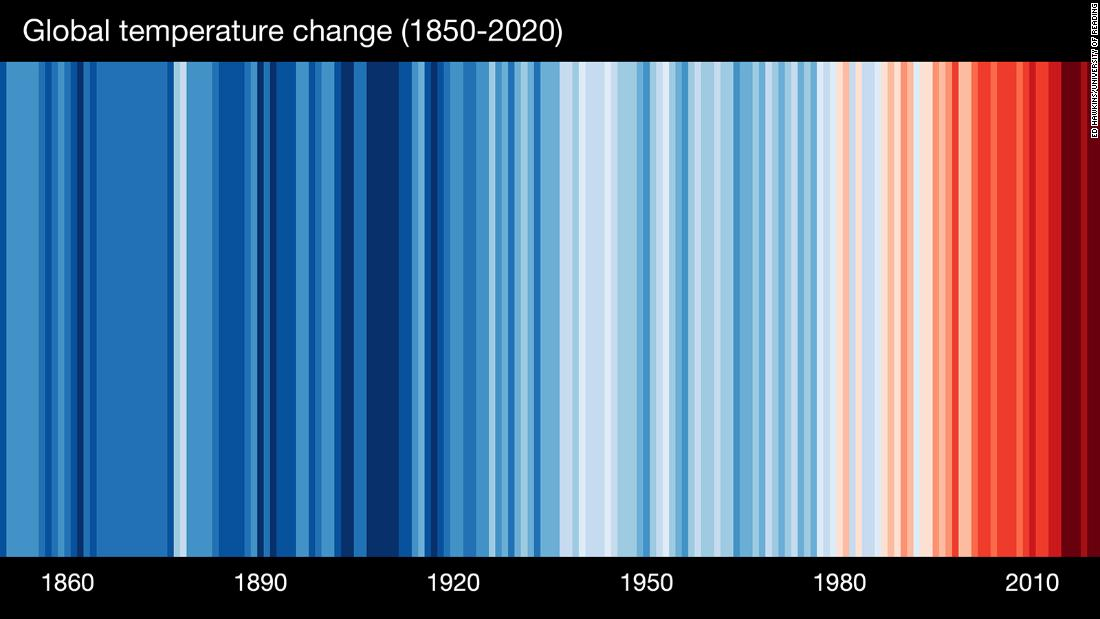
\includegraphics[width=.9\linewidth]{Figures/global-warming-graph.jpg}
%
%    \vspace{5mm}
%
%    \begin{itemize}
%        \item Consensus sur le réchauffement lié aux activités humaines
%        \item Toutes les activités sont concernées
%    \end{itemize}
%\end{frame}


\begin{frame}{Durabilité}
  \begin{itemize}
    \item Selon les Nations Unies 
    \begin{itemize}
      \item Durabilité (\textit{sustainability}) : ``la satisfaction des besoins
      des générations présentes sans compromettre la capacité des générations
      futures à satisfaire leurs propres
      besoins''\footnote{\url{https://www.un.org/fr/impact-universitaire/durabilit\%C3\%A9}}
    \end{itemize}
    \item Durabilité n'est pas uniquement liée aux impacts environnementaux    
    \item \textbf{Objectifs de développement durable :} cadre d'objectifs pour améliorer
    la vie des gens dans le monde entier et atténuer les effets de l'homme sur
    le climat.    
  \end{itemize}
  \centering 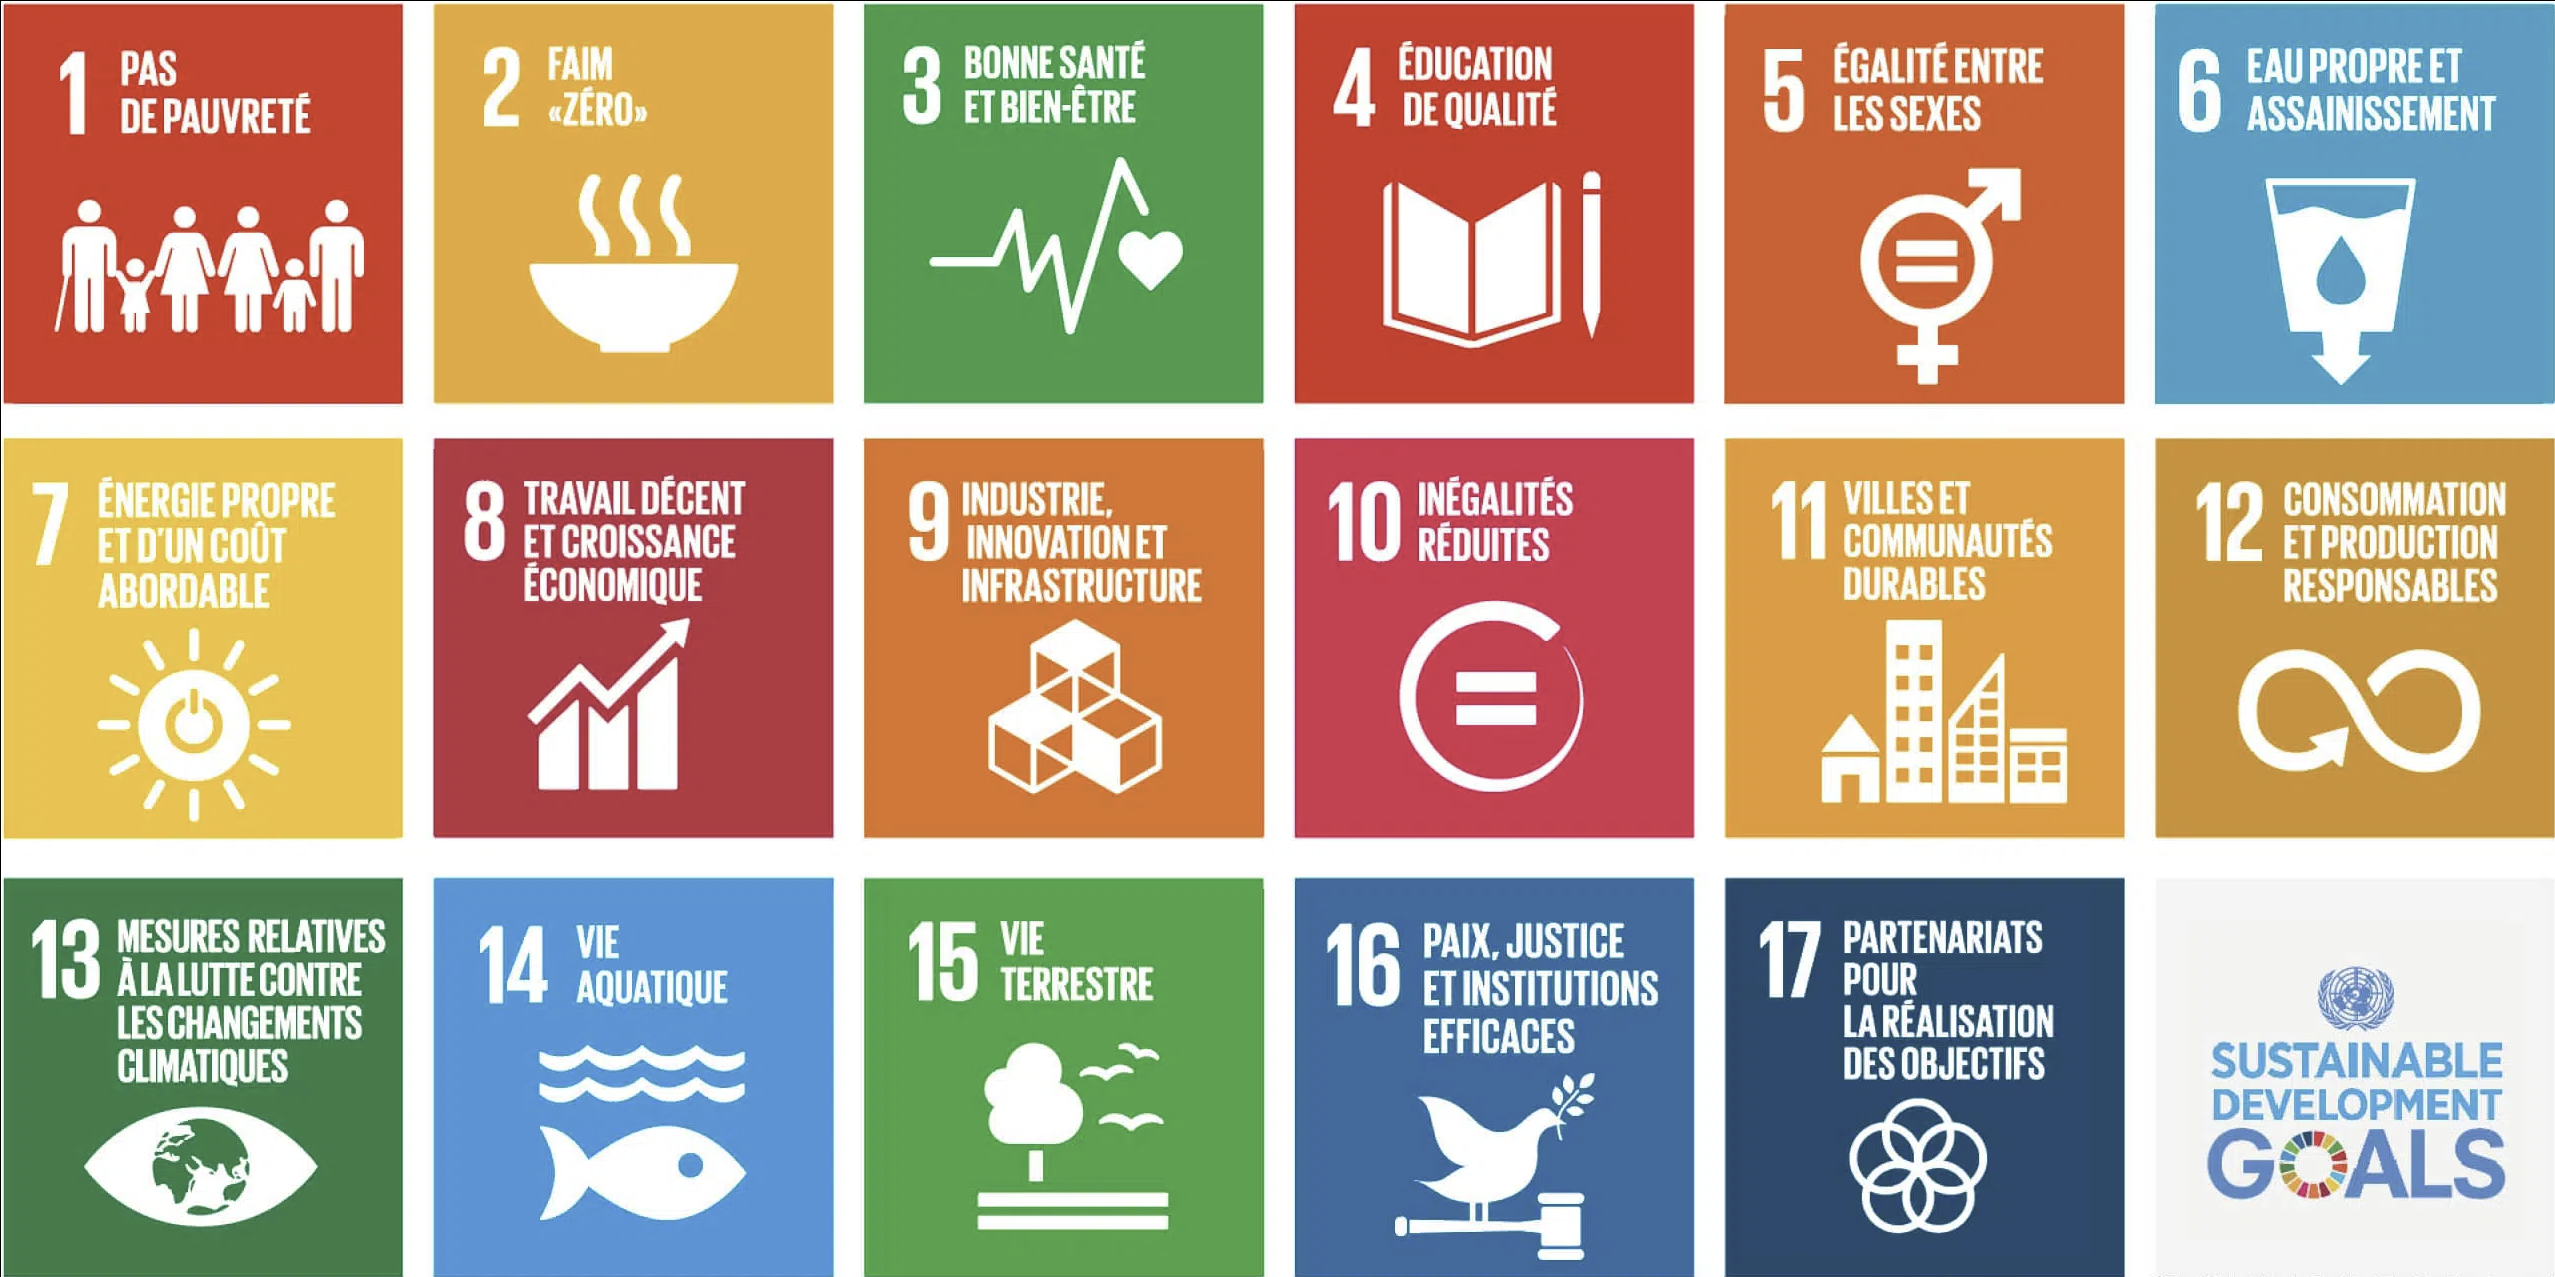
\includegraphics[width=.6\linewidth]{Figures/sdgs.png}
\end{frame}

\begin{comment} 

\begin{frame}{Durabilité}
  \begin{itemize}
    \item Une définition inventée par les Nations Unies 
    \begin{itemize}
      \item Durabilité (\textit{sustainability}) : ``la satisfaction des besoins
      des générations présentes sans compromettre la capacité des générations
      futures à satisfaire leurs propres
      besoins''\footnote{\url{https://www.un.org/fr/impact-universitaire/durabilit\%C3\%A9}}
    \end{itemize}
    \item \textbf{Objectifs de développement durable :} cadre d'objectifs pour améliorer
    la vie des gens dans le monde entier et atténuer les effets de l'homme sur
    le climat.    
  \end{itemize}
  \centering 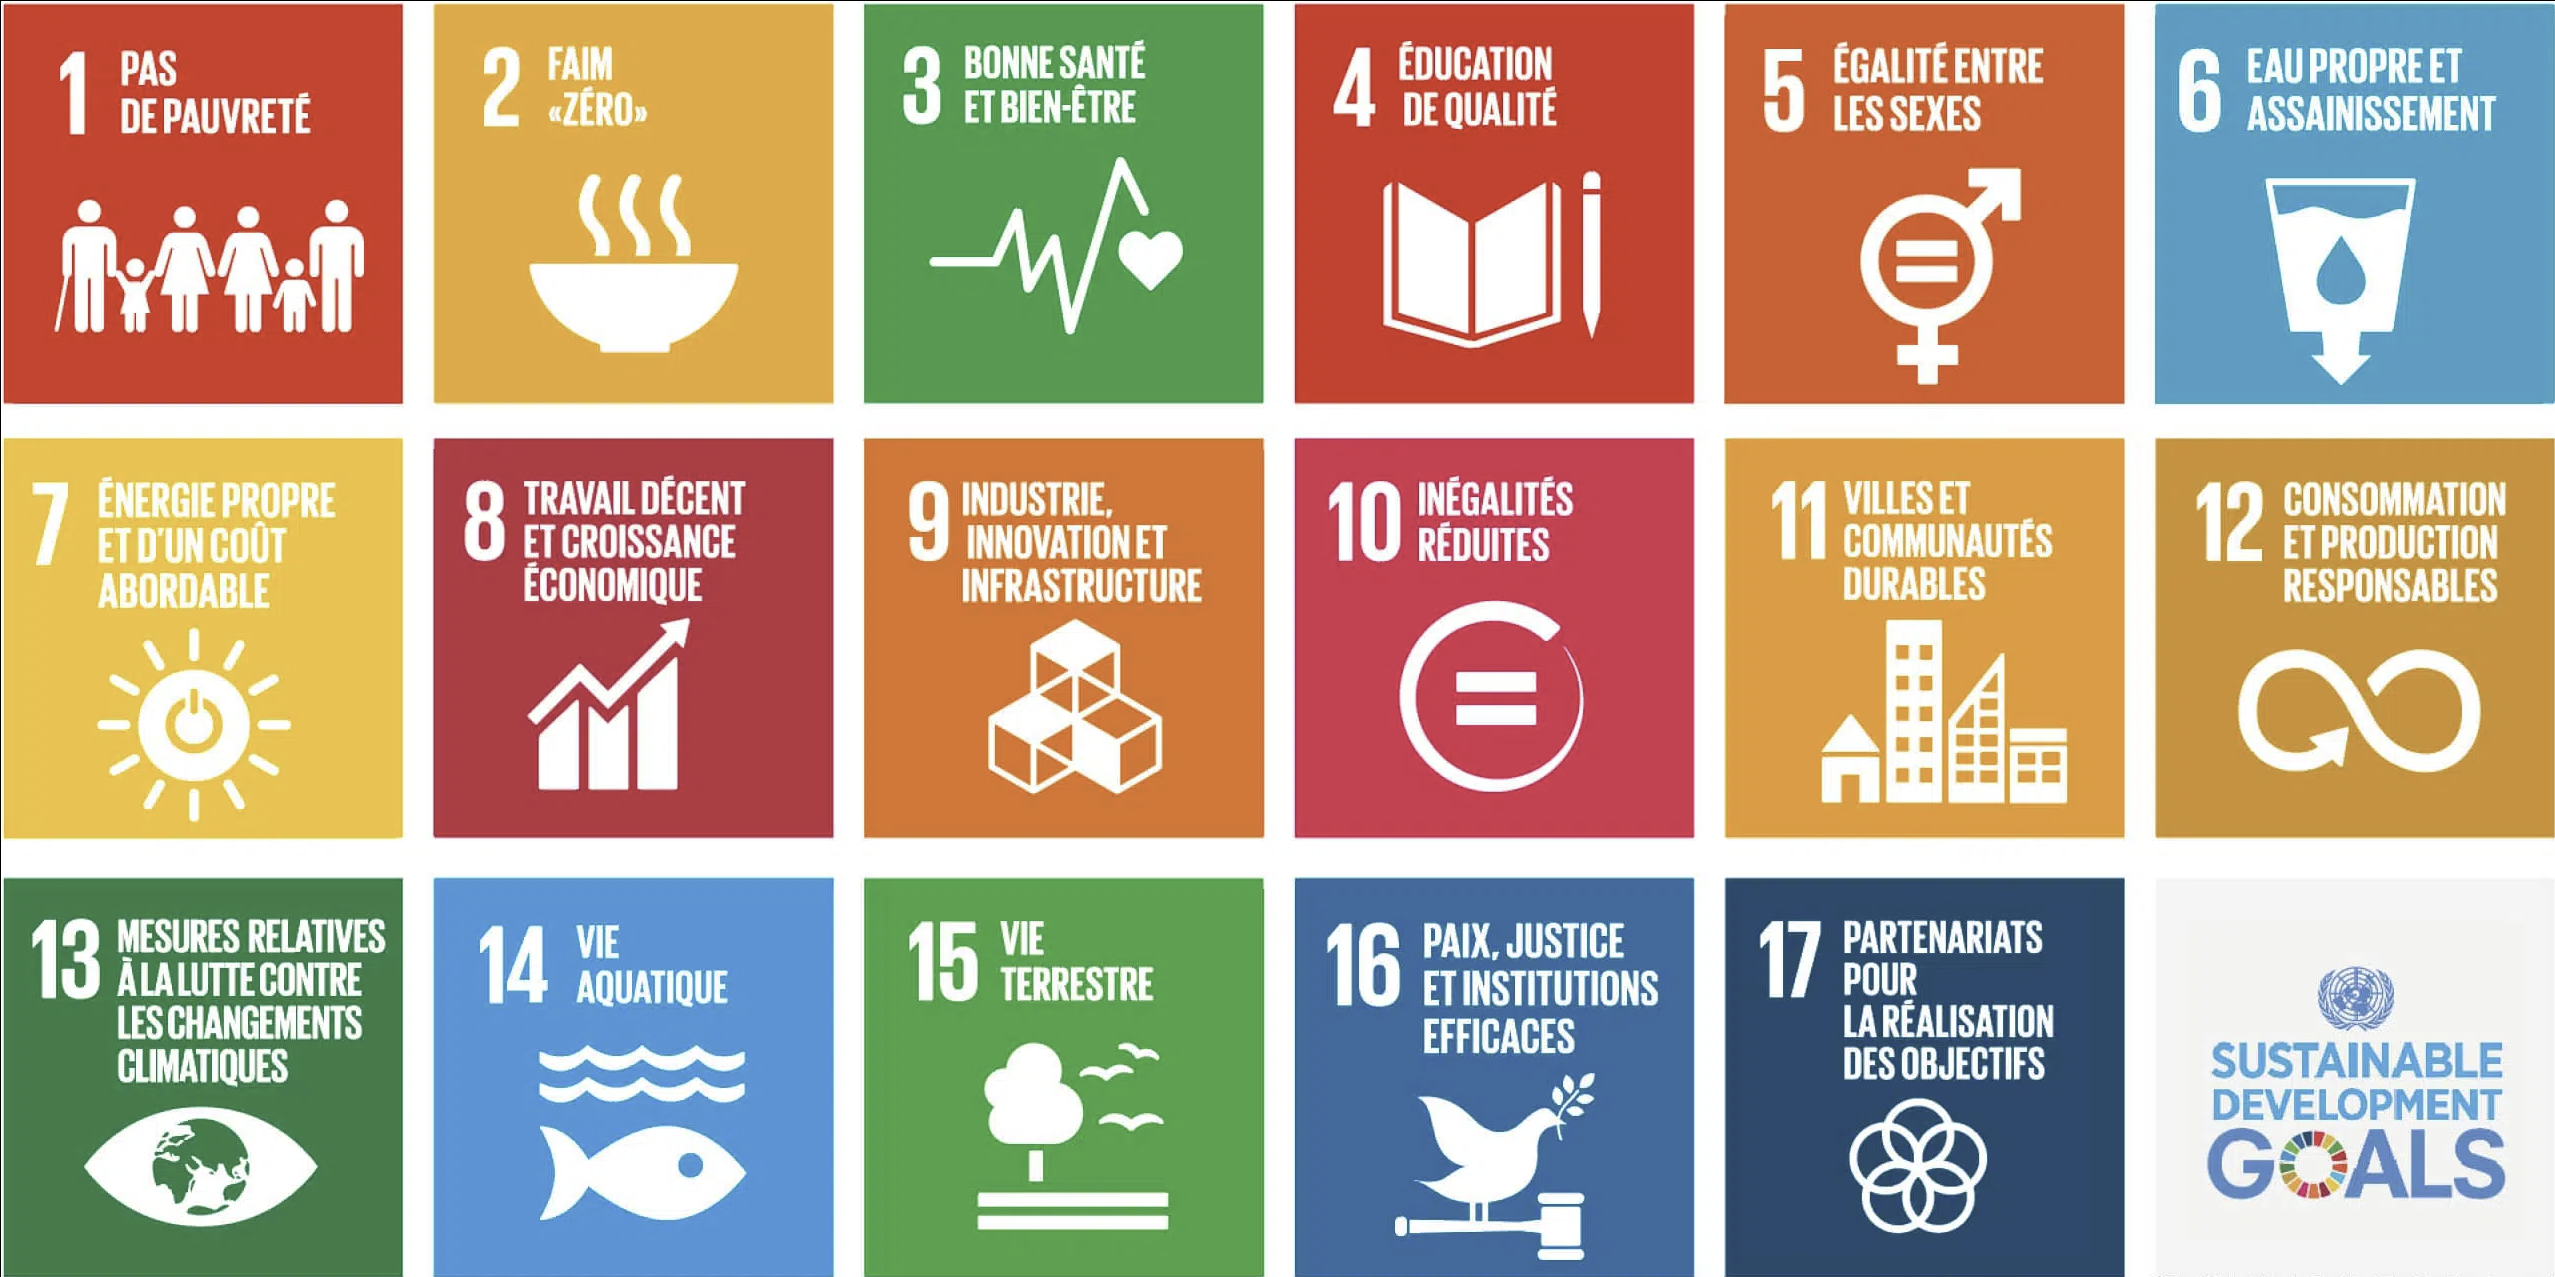
\includegraphics[width=.7\linewidth]{Figures/sdgs.png}
\end{frame}

\begin{frame}{Durabilité et impact environnemental}
  \begin{itemize}
    \item Durabilité n'est pas uniquement liée aux impacts environnementaux
    \begin{itemize}
      \item Environnement : ODDs 13 (Action sur le climat), 14 (Vie sous-marine)
      et 15 (Vie sur terre)      
    \end{itemize}
    \item ODDs : cadre important et très complexe, avec beaucoup de synergies et
    compromis.\footnote{Moallemi, E. A., Hosseini, S. H., Eker, S., Gao, L.,
    Bertone, E., Szetey, K., \& Bryan, B. A. (2022). Eight archetypes of
    sustainable development goal (SDG) synergies and trade-offs. Earth’s Future,
    10(9)}
  \end{itemize}

  \centering 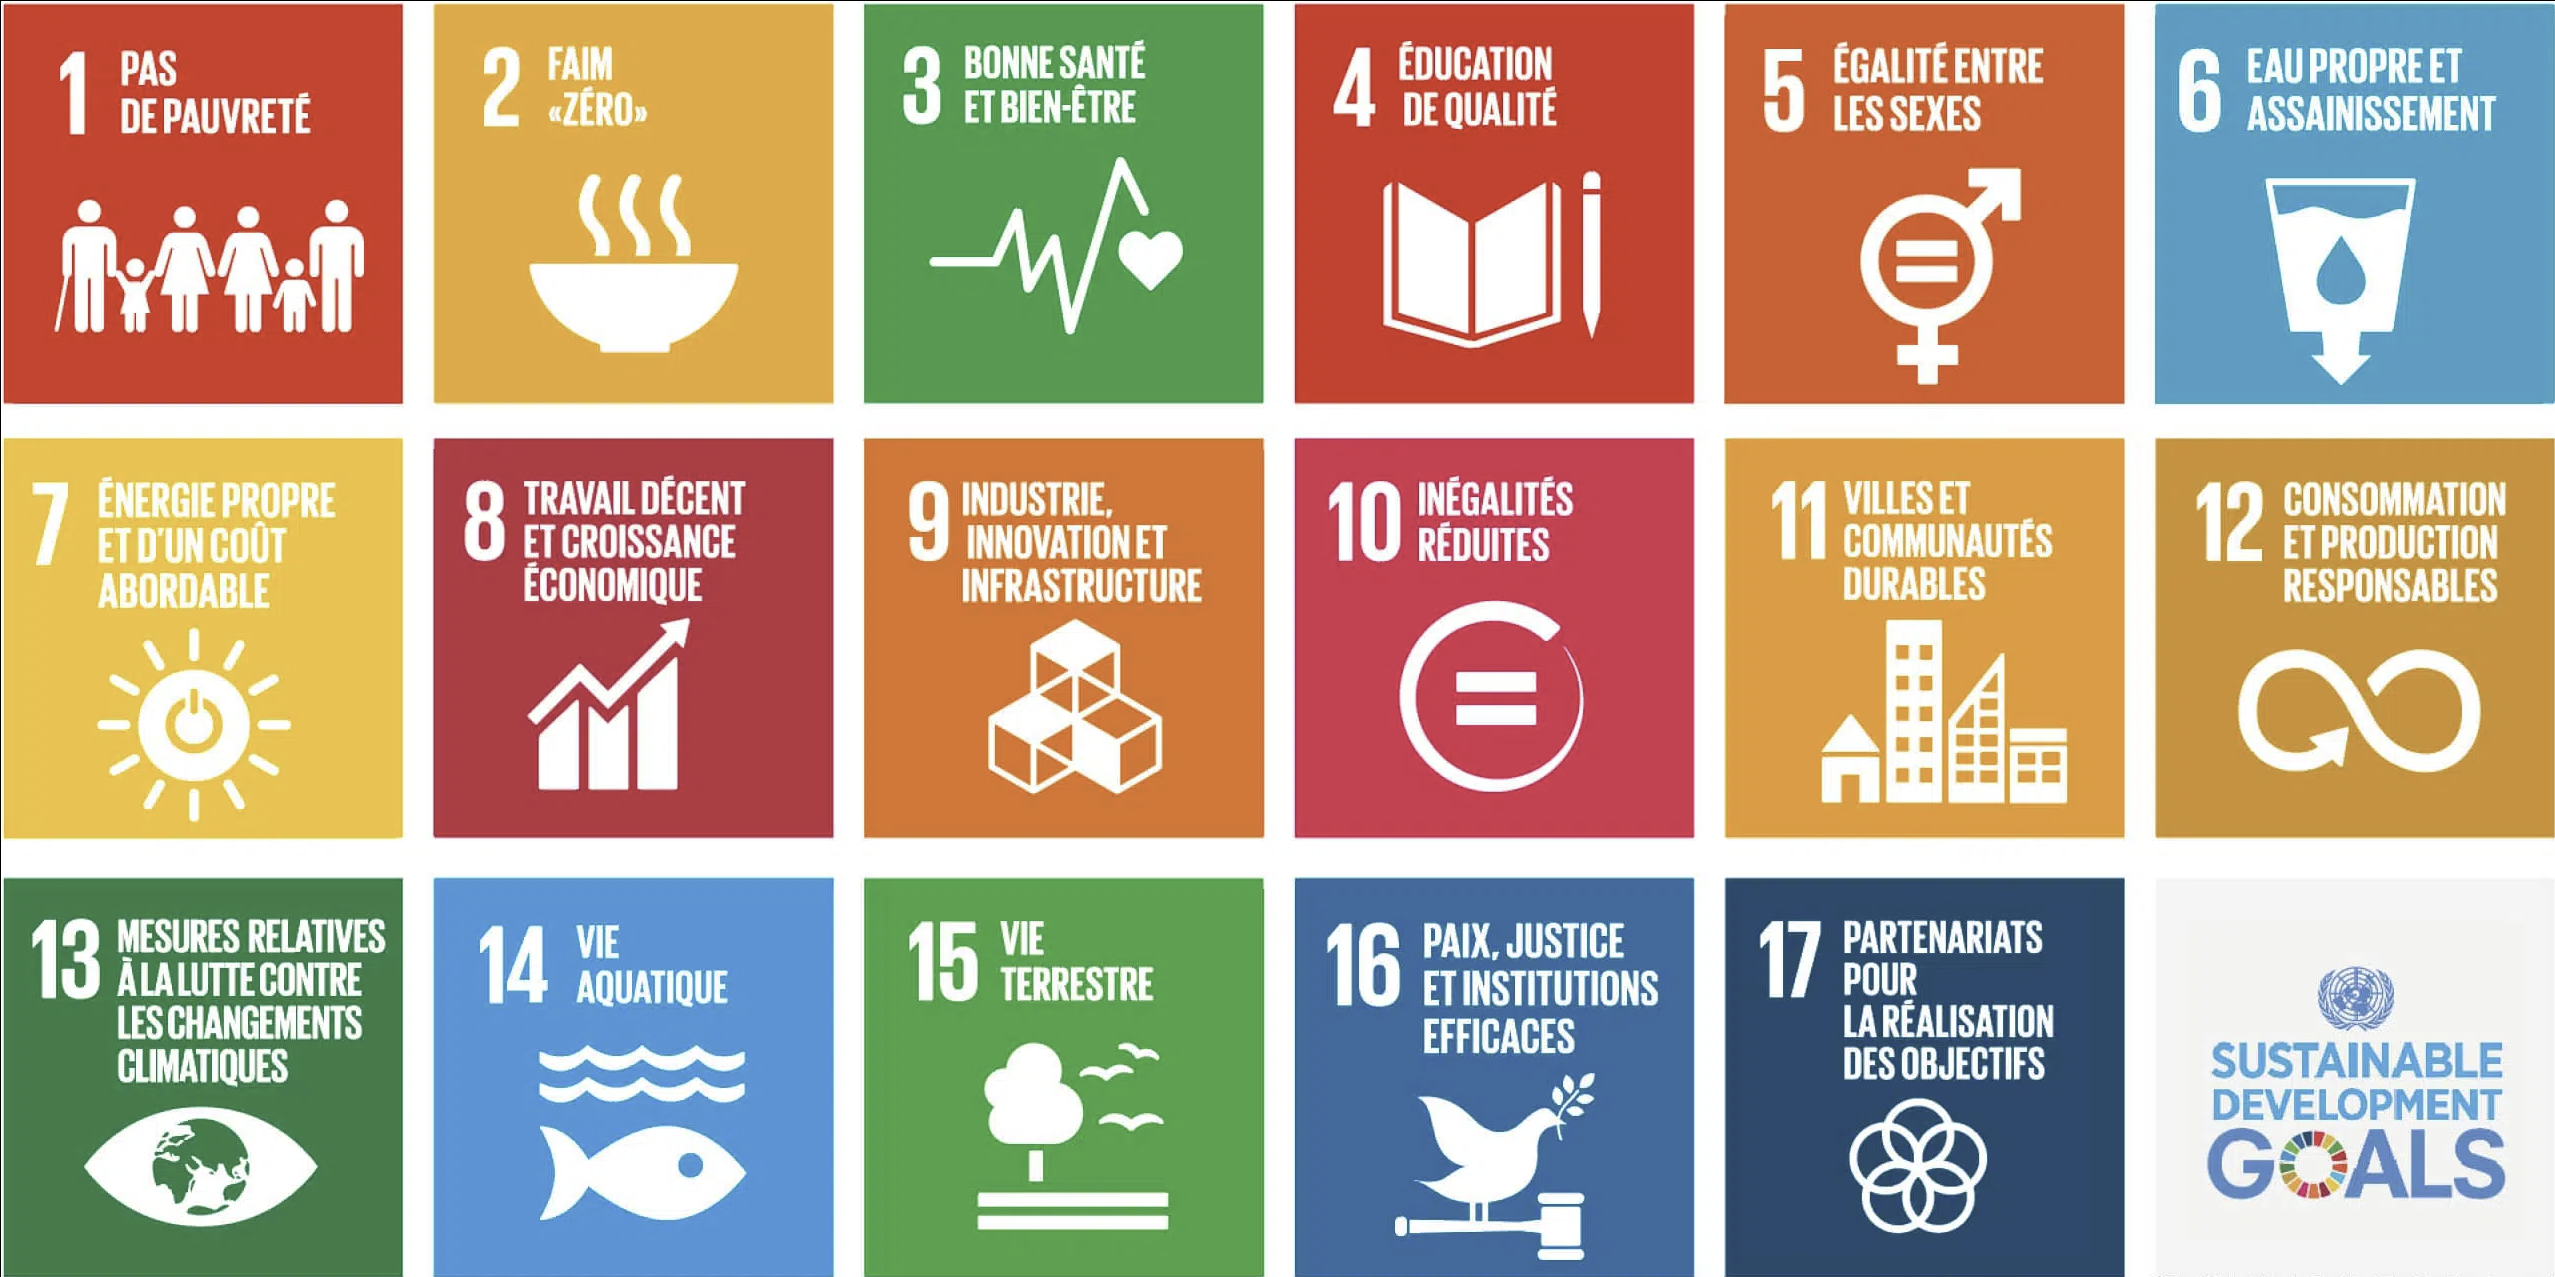
\includegraphics[width=.7\linewidth]{Figures/sdgs.png}
\end{frame}
\end{comment}

\begin{frame}{Les solutions numériques (y compris les solutions Cloud)}
  \begin{itemize}
    \item Cadre de technologies d'information et communication (\textit{Information and Communications Technologies}, ICT)
    \item Définition d'une solution numérique : \textit{``A system encompassing ICT
    goods, ICT networks and/or ICT services that contributes to meeting a
    technical, societal or business challenge''}\footnote{Recommendation L.1480 :
    \textit{Enabling the Net Zero transition: Assessing how the use of
    information and communication technology solutions impact greenhouse gas
    emissions of other sectors}. International Telecommunication Union (ITU).
    \url{https://www.itu.int/rec/T-REC-L.1480-202212-I}}
    \item Cela peut inclure : des logiciels, du matériel de traitement et de
    contrôle des données, infrastructure de réseau de télécommunications, un
    stockage de données, des écrans, et traitement de données à distance (centre
    de données et le \textbf{Cloud Computing}).
  \end{itemize}  
\end{frame}


\begin{frame}{Durabilité et le numérique}{Deux points de vue}
  
  \begin{enumerate}
    \item Numérique comme solution
    \begin{itemize}
      \item Transition écologique par la transition numérique (\textit{digital
      transition}) : le numérique pour optimiser l'utilisation de ressources
      des activités humaines
      \begin{itemize}
        \item Exemple : réunion en visioconférence au lieu qu'en présentiel
      \end{itemize}
    \end{itemize}
    \item Numérique comme problème
    \begin{itemize}
      \item Illusion du ``dématérialisé'', ce qui n'est pas physique, virtuel, coût zéro
      \begin{itemize}
        \item Le numérique est pourtant bien physique et consommateur de ressources
      \end{itemize} 
      \item Accélérateur des nouvelles modes de consommation et d'usage
      \begin{itemize}
        \item Exemple :
        \textit{streaming}\footnote{\url{https://youtu.be/whML39I7Q7Y?t=1593}}
        et publicité ciblée par systèmes de recommandation
      \end{itemize}
    \end{itemize}    
  \end{enumerate}
  \begin{itemize}
    \item Les deux points de vue s'entremêlent
  \end{itemize}
  
\end{frame}

\begin{frame}{Focus sur l'impact environnemental}
  \begin{itemize}
    \item Synthèse sur les composants principaux :
    \begin{enumerate}
      \item Indicateurs d'impact
      \item Phases du cycle de vie
      \item Périmètre 
    \end{enumerate}
  \end{itemize}
\end{frame}

\begin{frame}{Indicateurs d'impact}{Quelques exemples}
  \begin{itemize}
    \item Les plus souvent utilisés
    \begin{enumerate}
      \item Consommation d'énergie primaire (électricité, carburants)
      \item Changement climatique (émissions de gaz à effet de serre)
    \end{enumerate}
    \item Moins souvent utilisés, mais également importants
    \begin{enumerate}
      \item Utilisation d'eau
      \item Épuisement des ressources abiotiques : Épuisement
      des ressources naturelles non fossiles (métaux rares)
      \item Radiations ionisantes : Dommages à la santé humaine et aux
      écosystèmes liés aux émissions de radionucléides
    \end{enumerate}
  \end{itemize}  
\end{frame}

\begin{frame}{Indicateurs d'impact}{Changement climatique}
\begin{itemize}
  \item Mesuré en kilogrammes de CO2 équivalent émit dans l'atmosphère
  \item Équivalent CO2 : 
  \begin{itemize}
    \item Il existe plusieurs gaz à effet de serre, avec un potentiel de
    réchauffement global (\textit{global warming
    potential\footnote{\url{https://fr.wikipedia.org/wiki/Potentiel_de_r\%C3\%A9chauffement_global}}},
    GWP) spécifique
    \item CO2 est la référence (GWP = 1). 
    \item Un gaz avec un GWP = 2 signifie qu'il a deux fois plus de potentiel de
    réchauffement global
    \item Exemples de GWP : protoxyde d'azote (N2O) = 273
    \begin{itemize}
      \item 1 kg de protoxyde d'azote émit dans l'air équivaut à 273 kg de CO2
      émit dans l'air
    \end{itemize} 
  \end{itemize}
\end{itemize}
\end{frame}

\begin{frame}{Émissions liées à l'électricité}{Mix énergétique}
  \begin{enumerate}
    \item \url{https://ourworldindata.org/electricity-mix}
    \item \url{https://app.electricitymaps.com/map/24h}
  \end{enumerate}  
\end{frame}

\begin{frame}{Phases du cycle de vie}
  \begin{columns}
    \begin{column}{.5\textwidth}
      \centering 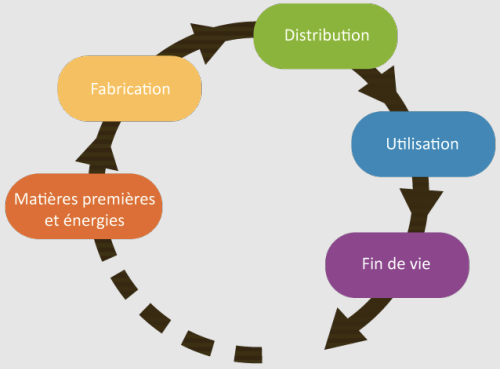
\includegraphics[width=\linewidth]{Figures/life-cycles.png}
    \end{column}
    \begin{column}{.5\textwidth}
      \begin{itemize}
        \item Phase d'utilisation est largement prise en compte. 
        \item Les autres phases sont souvent négligées
        \item \textbf{Question :} Quelles parties d’une solution numérique
        appartiennent à quelle phase du cycle de vie ? 
      \end{itemize}
    \end{column}
  \end{columns}  
\end{frame}

\begin{frame}{Périmètre}
  Deux concepts :
  \begin{enumerate}
    \item Scope
    \begin{itemize}
      %\item Souvent utilisé pour l'émission de CO2, mais le principe s'applique
      %aussi à d'autres indicateurs
      \item Scope 1 : Émissions directes provenant de sources détenues ou
      contrôlées
      \item Scope 2 : Émissions liées à la consommation d'énergie
      \item Scope 3 : Émissions liées à la chaine de valeur
    \end{itemize}
    \item Ordre\footnote{\url{https://www.greendigitalcoalition.eu/assets/uploads/2024/04/EGDC-Net-Carbon-Impact-Assessment-Methodology-for-ICT-Solutions.pdf}}
    \begin{itemize}
      \item Prermier ordre : Impacts liés au cycle de vie de la solution
      \item Deuxième ordre : Conséquences directes après le déploiement de la solution
      \item Effets d'ordre supérieure : Conséquence d'impacts de deuxième ordre,
      souvent dû aux changements de modes de consommation, de comportement,
      style de vie, etc. Effets rebond.
    \end{itemize}
  \end{enumerate}
\end{frame}

\begin{frame}{Mise en situation}{Développement d'une plate-forme de \textit{streaming} (1 sur 3)}
  \begin{itemize}
    \item Indicateur : émissions de CO2
    \item Phases du cycle de vie
    \begin{itemize}
      \item \textbf{Matières premières :} extraction de métaux pour fabriquer
      l'infrastructure informatique (serveurs, réseau, etc.)
      \item \textbf{Fabrication :} manufacture du matériel informatique (CPU, mémoire,
      stockage, GPU, routeurs réseau, fibre optique, tours réseau mobile)
      \item \textbf{Distribution :} livraison du matériel informatique
      \item \textbf{Utilisation :} électricité consommée pendant le par la
      plate-forme (développement + usage par les clients + infrastructure
      réseau) multipliée par le mix énergétique de l'électricité
      \item \textbf{Fin de vie :} élimination ou recyclage de du matériel informatique
    \end{itemize}
  \end{itemize}  
\end{frame}

\begin{frame}{Mise en situation}{Développement d'une plate-forme de \textit{streaming} (2 sur 3)}
  \begin{itemize}
    \item Périmètre
    \begin{itemize}
      \item \textbf{Scope 1 :} Pas d'émissions
      \item \textcolor{red}{\textbf{Scope 2 :}}\footnote{Scope 2 est le
      composant le plus pris en compte actuellement} Émissions liées à la
      consommation d'électricité du développement + potentiel hébergement du
      service sur place (phase d'utilisation)
      \item \textbf{Scope 3 :} Émissions liées à l'électricité consommée par les clients, infrastructure
      réseau et hébergement externe (phase d'utilisation). Émissions liées aux phases matières premières, fabrication et fin de vie
    \end{itemize}    
  \end{itemize}
\end{frame}

\begin{frame}{Mise en situation}{Développement d'une plate-forme de \textit{streaming} (3 sur 3)}
  \begin{itemize}
    \item Ordre
    \begin{itemize}
      \item \textbf{Premier ordre :} Émissions liées à tous les composants mentionnés dessus
      \item \textbf{Deuxième ordre :} Émissions liées à la consommation des médias
      physiques (DVD) (réduction d'émissions). Émissions liées à la demande des
      clients (augmentation d'émissions)
      \item \textbf{Effets d’ordre supérieur :} Émissions liées aux changements de comportement induits par le service :
      \begin{itemize}
        \item Streaming sur téléphone portable + réseau mobile
        \item Addiction aux vidéos courtes
        \item Consommation induite par la publicité ciblée, via des publicités
        intégrées dans le service ou des influenceurs
        \item Changement d'infrastructure pour répondre à la demande (4G $\rightarrow$ 5G $\rightarrow$ 6G $\rightarrow$ ...)
      \end{itemize}
    \end{itemize}
  \end{itemize}
\end{frame}

\begin{frame}{L'effet rebond}
  \begin{itemize}
    \item Concept provenant du domaine de l'économie : Paradoxe de
    Jevons\footnote{\url{https://fr.wikipedia.org/wiki/Paradoxe_de_Jevons}}

    \item À mesure que les améliorations technologiques augmentent
    l'efficacité avec laquelle une ressource est employée, la consommation
    totale de cette ressource peut augmenter au lieu de diminuer

    \item Pensée générale : un service est plus efficace $\rightarrow$ le
    service devient moins cher/plus pratique/plus attractif $\rightarrow$ le
    service est plus utilisé $\rightarrow$ la consommation de ressources
    augmente

    \item \textbf{Question ouverte :} Trouver un service numérique où des
    optimisations particulières n'ont pas été accompagnées d'effets
    rebond\footnote{\url{https://cacm.acm.org/opinion/let-us-not-put-all-our-eggs-in-one-basket/}}
  \end{itemize}  
\end{frame}

\begin{frame}{Les outils existants (1 sur 2)}
  \begin{itemize}
    \item Phase d'utilisation (consommation électrique dans l'infrastructure informatique sur place)
    \begin{itemize}
      \item Wattmètres physiques et logiciels\footnote{Contenu abordé en détail
      dans l'UE Eco-Conception Web en M2 MIAGE}
      \begin{itemize}
        \item Possible uniquement sur en Cloud privé ou sur un service IaaS
        (\textit{infrastructure as a service})
      \end{itemize}      
    \end{itemize}
    \item Les autres phases
    \begin{itemize}
      \item Base IMPACTS numérique de l'ADEME\footnote{\url{https://base-empreinte.ademe.fr/documentation/base-impact?idDocument=167}}
      \item Datavizta\footnote{\url{https://dataviz.boavizta.org/}}
      \item Ecoinvent\footnote{\url{https://ecoinvent.org/}} (base payante)
      \item Certaines phases, notamment la fin de vie et distribution (transport), parfois ne sont pas prises en compte
    \end{itemize}       
  \end{itemize}
  
\end{frame}

\begin{frame}{Les outils existants (2 sur 2)}
  \begin{itemize}
    \item Les effets d'ordre supérieur et effets rebond
    \begin{itemize}
      \item Analyses qualitatives \textit{ad-hoc} (évaluation au cas par cas)
      \item Domaine de recherche récent
    \end{itemize} 
    \item Services fournis par les \textit{hyperscalers}
    \begin{itemize}
      \item AWS : Customer carbon footprint tool\footnote{\url{https://aws.amazon.com/fr/aws-cost-management/aws-customer-carbon-footprint-tool/}}
      \item GCP : Carbon footprint\footnote{\url{https://cloud.google.com/carbon-footprint}}
      \item Azure : Emissions impact dashboard\footnote{\url{https://www.microsoft.com/en-us/sustainability/emissions-impact-dashboard}}
      \item \textbf{Question :} Quels sont les indicateurs et le périmètre couverts par les services des hyperscalers ?
    \end{itemize}
  \end{itemize}
\end{frame}

\begin{frame}{Que peut-on faire ?}{Quelques pistes}

  \begin{itemize}
    \item Interroger la pertinence des solutions
    \begin{itemize}
      \item Trop futile ? Trop gadget ?
      \item Risque de surconsommation/superattractivité/addiction ?
    \end{itemize}
    \item Mesurer et estimer les impacts dans tout le cycle de vie et le
    périmètre le plus large possible
    \item Informer les utilisateurs/clients de ces mesures et estimations
    \item Éviter de : 
    \begin{itemize}
      \item Promettre une livraison de service immédiate, quel que soit le nombre de clients et d'usages
      \item Promettre un stockage illimité dans l'espace et dans le temps 
      \item Supposer la disponibilité éternelle de certains matériels, logiciels et fournisseurs cloud
      \item Concevoir des services permettant des extensions fonctionnelles illimitées
    \end{itemize}
  \end{itemize}
  
\end{frame}

\begin{frame}{Contenu Supplémentaire}
  \begin{scriptsize}
    \begin{itemize}
      \item International Telecommunication Union (ITU). L.1480 : Enabling the Net
      Zero transition: Assessing how the use of information and communication
      technology solutions impact greenhouse gas emissions of other sectors
      (2022)\footnote{\url{https://www.itu.int/rec/T-REC-L.1480-202212-I}}      
      \item European Green Digital Coalition (EGDC). Net-Carbon Impact Assessment
      Methodology (2024)\footnote{\url{https://www.greendigitalcoalition.eu/net-carbon-impact-assessment-methodology-for-ict-solutions/}}
      \item Perasso, E. L., Vateau, C., \& Domon, F. (2022). Evaluation de
      l’impact environnemental du numérique en France et analyse prospective.
      ADEME\footnote{\url{https://www.arcep.fr/uploads/tx\_gspublication/etude-numerique-environnement-ademe-arcep-volet02\_janv2022.pdf}}
      \item Maraninchi, F. (2022). Let us not put all our eggs in one basket. Communications of the ACM, 65(9), 35-37      
    \end{itemize}
  \end{scriptsize} 
\end{frame}

% interroger la pertinance des solutions (trop futile ? trop gadget ? risque de surconsommation/surattrativité/addiction ?)
% mesurer et estimer les impacts dans tout le cycle de vie et le périmètre le plus large possible
% informer les clients des mesures et estimations
% fournir des solutions alternatives plus frugales en option, même si ces solutions dégradent la qualité du service
% optimiser les solutions (le moindre consommation électrique, choix de data centre )

% ITU-T L.1480, direct rebound effect: A rebound effect where increased efficiency, associated cost
%reduction and/or convenience of a product or service results in its increased use because it is
%cheaper or otherwise more convenient. 

% Notre maison brûle et nous regardons ailleurs. ... Nous ne pourrons pas dire que nous ne savions pas. Jacques Chirac

% futile, gadget ?

%https://www.greendigitalcoalition.eu/assets/uploads/2024/04/EGDC-Net-Carbon-Impact-Assessment-Methodology-for-ICT-Solutions.pdf

\end{document}